\section{Вычислительный эксперимент}
\subsection{Условия проверки}
Для каждого размера \texttt{n} создаётся список \texttt{data}
из последовательных целых чисел от нуля до \texttt{n - 1}.
Искомому значению \texttt{target} присваивается \texttt{n}.
Такого значения в списке нет, поэтому оба алгоритма должны вернуть
индекс \texttt{-1}. Счётчик \texttt{steps} увеличивается один раз
за итерацию основного цикла.

Полная программа приведена в приложении~\ref{app:source},
в листингах~\ref{code:search} и~\ref{code:experiment}.
Функции возвращают пару: индекс найденного элемента и число шагов.
Для бинарного поиска предполагается, что список уже отсортирован;
затраты на подготовку списка в результаты не включены.

В Python функция \texttt{bisect\_left} модуля \texttt{bisect} использует
похожий принцип, но возвращает позицию вставки. Наличие значения нужно
проверять отдельно~\cite{python}.

\subsection{Полученные результаты}
В таблице~\ref{tab:results} приведены результаты запуска программы.
Для выбранного значения, превышающего все элементы, бинарный поиск
достигает оценки \eqref{eq:binary}.
\begin{table}[H]
\centering
\caption{Число шагов при поиске отсутствующего значения}
\label{tab:results}
\begin{tabular}{|r|r|r|}
\hline
Размер \texttt{n} & Линейный поиск & Бинарный поиск \\
\hline
8 & 8 & 4 \\
16 & 16 & 5 \\
32 & 32 & 6 \\
64 & 64 & 7 \\
128 & 128 & 8 \\
256 & 256 & 9 \\
512 & 512 & 10 \\
1024 & 1024 & 11 \\
\hline
\end{tabular}
\end{table}

На рисунке~\ref{fig:steps} показано изменение числа шагов при увеличении
размера списка. Логарифмическая шкала вертикальной оси позволяет видеть
обе зависимости на одном графике. Графики построены по результатам программы.
\begin{figure}[H]
\centering
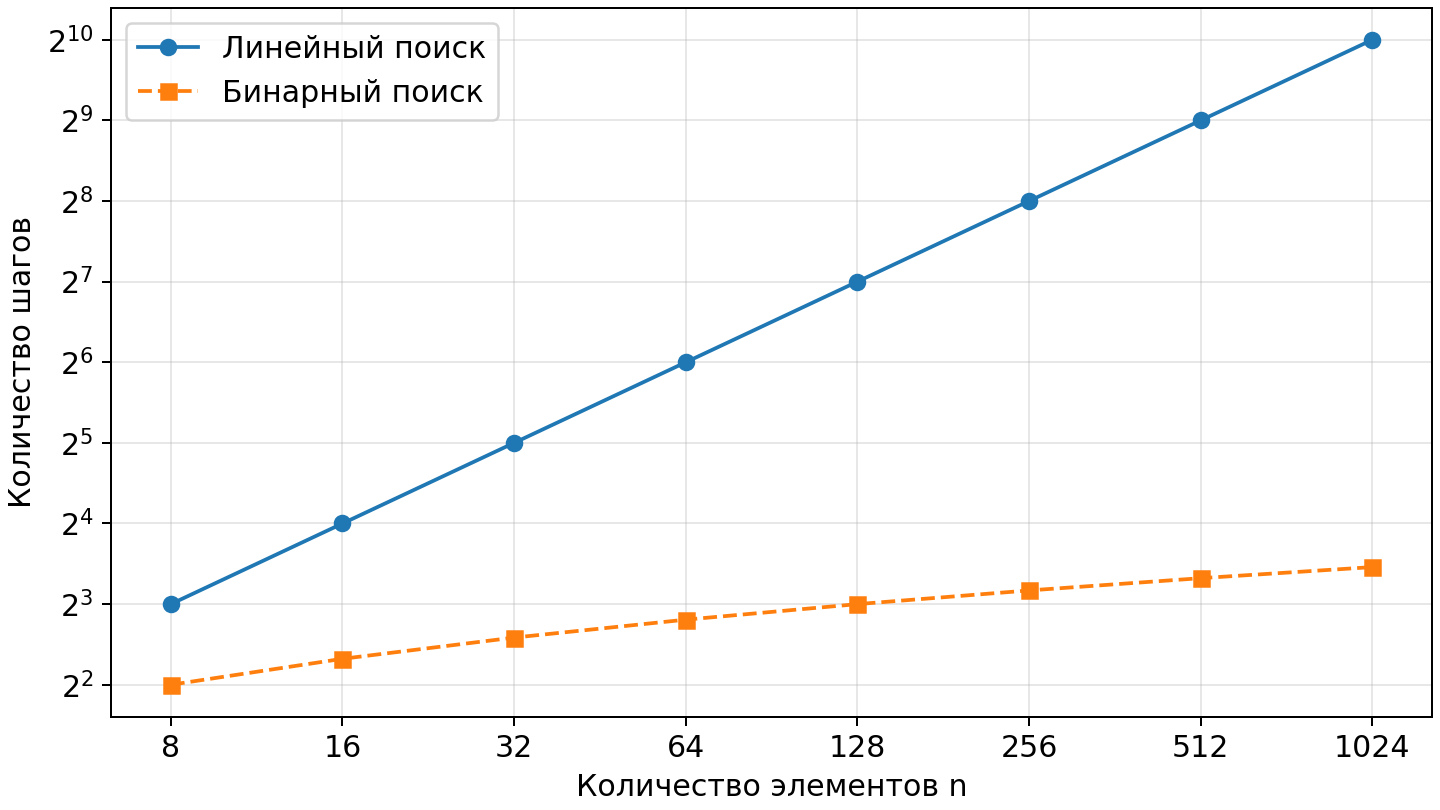
\includegraphics[width=0.82\textwidth]{images/steps.png}
\caption{Число шагов двух алгоритмов}
\label{fig:steps}
\end{figure}

Для сравнения введём отношение числа шагов:
\begin{equation}
\mathtt{K}(\mathtt{n})=
\frac{\mathtt{L}(\mathtt{n})}{\mathtt{B}(\mathtt{n})}.
\label{eq:ratio}
\end{equation}
Здесь \texttt{B(n)} --- число шагов бинарного поиска в эксперименте.
Для размера \texttt{n = 1024} отношение составляет
\(\mathtt{K}(1024)=1024/11\approx 93{,}09\).
Это отношение количества итераций, а не измеренное ускорение программы.

На рисунке~\ref{fig:ratio} видно, как увеличивается отношение
\eqref{eq:ratio}. При переходе от 512 к 1024 элементам линейный поиск
выполняет вдвое больше шагов, а бинарный --- всего на один шаг больше.
\begin{figure}[H]
\centering
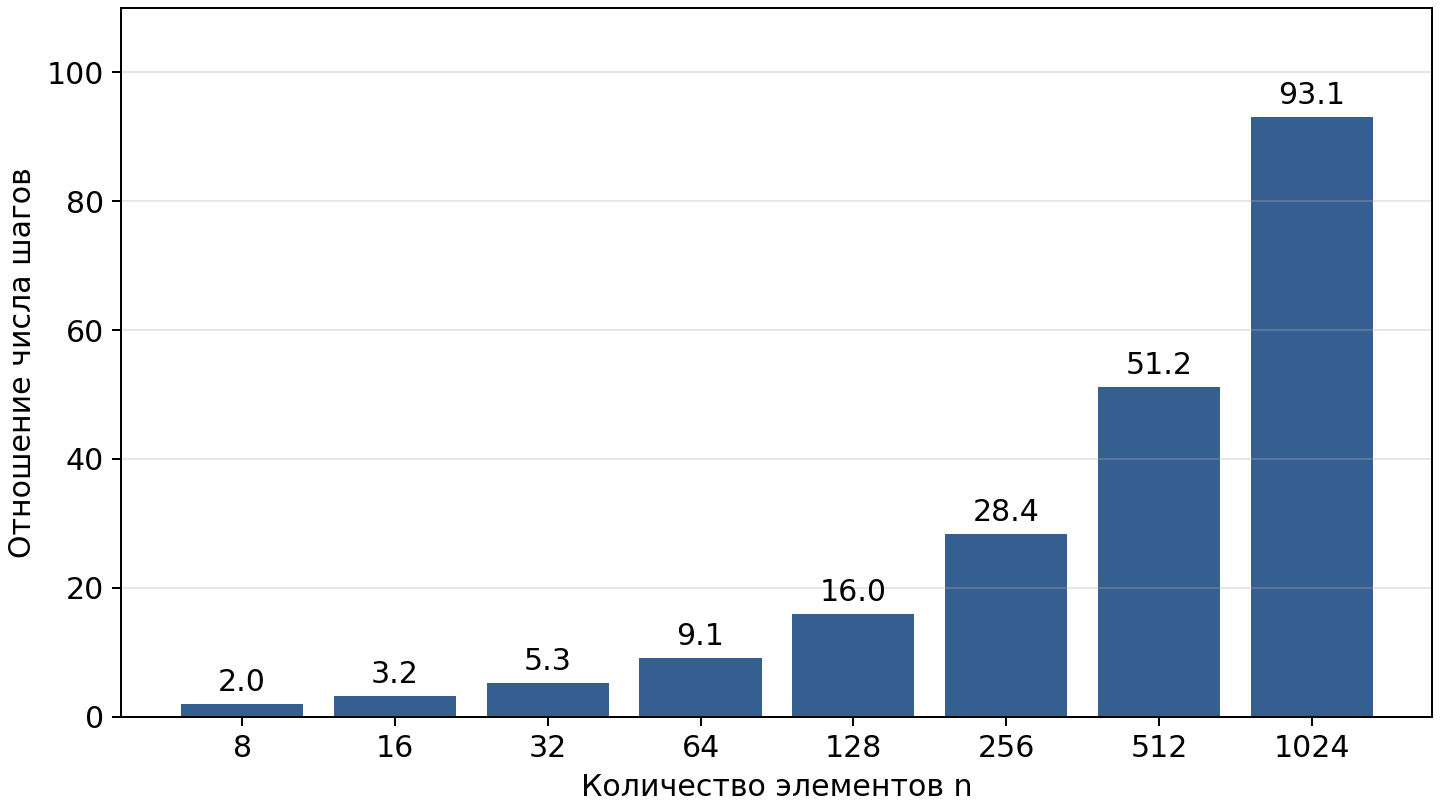
\includegraphics[width=0.82\textwidth]{images/ratio.png}
\caption{Отношение числа шагов линейного и бинарного поиска}
\label{fig:ratio}
\end{figure}

\subsection{Ограничения сравнения}
В опыте рассмотрен один вид запроса: отсутствующее значение больше всех
элементов списка. Для другого запроса количество шагов может измениться.
Например, линейный поиск найдёт первый элемент за один шаг.

Бинарный поиск удобен, когда данные уже упорядочены и обращения по индексу
быстрые. Если требуется только один поиск в неупорядоченных данных,
предварительная сортировка может оказаться лишней работой.
Поэтому результат эксперимента не означает, что бинарный поиск всегда
лучше при любых условиях.
